\documentclass[11pt,a4paper]{article}
\usepackage[T1]{fontenc}
\usepackage[utf8]{inputenc}
\usepackage{lmodern}
\usepackage[margin=22mm,headheight=16pt]{geometry}
\usepackage{amsmath,amssymb,graphicx,array,longtable,booktabs}
\usepackage{microtype,xcolor,hyperref,xurl,fancyhdr}
\definecolor{Navy}{HTML}{17324D}
\definecolor{Teal}{HTML}{087F8C}
\definecolor{Gold}{HTML}{B88128}
\hypersetup{colorlinks=true,linkcolor=Navy,urlcolor=Teal,bookmarksnumbered=true,hypertexnames=false}
\setlength{\parindent}{0pt}
\setlength{\parskip}{6pt}
\setlength{\emergencystretch}{4em}
\setcounter{tocdepth}{1}
\pagestyle{fancy}\fancyhf{}
\fancyfoot[R]{\small\thepage}
\fancyfoot[L]{\small\sffamily Sharif University of Technology}
\renewcommand{\headrulewidth}{0.3pt}
\makeatletter
\renewcommand\section{\@startsection{section}{1}{\z@}{-3.2ex plus -1ex minus -.2ex}{1.6ex plus .2ex}{\normalfont\Large\sffamily\bfseries\color{Navy}}}
\renewcommand\subsection{\@startsection{subsection}{2}{\z@}{-2.5ex plus -1ex minus -.2ex}{1.2ex plus .2ex}{\normalfont\large\sffamily\bfseries\color{Teal}}}
\makeatother
\fancyhead[L]{\small\sffamily\color{Navy}Reza Sanaee Nezhad}\fancyhead[R]{\small\sffamily\color{Teal}Technical Report}\begin{document}
\begin{titlepage}\centering\vspace*{7mm}

\includegraphics[width=31mm]{assets/sharif_emblem_en.png}\par\vspace{5mm}
{\Large\sffamily\bfseries\color{Navy}SHARIF UNIVERSITY OF TECHNOLOGY\par}
\vspace{2mm}{\sffamily Department of Electrical Engineering\par}
\vspace{17mm}{\color{Teal}\rule{\linewidth}{1.4pt}}\par\vspace{6mm}
{\large\sffamily\color{Teal}TECHNICAL REPORT\par}
\vspace{8mm}{\huge\sffamily\bfseries\color{Navy}Distributed Sensor Monitoring with HTTP, MQTT, SNMP, and SQLite\par}
\vspace{9mm}{\color{Gold}\rule{45mm}{1pt}}\par\vfill
\begin{minipage}{.88\linewidth}{\sffamily\color{Teal}AUTHOR}\par{\Large\sffamily Reza Sanaee Nezhad}\par Student ID: 401101502\par\vspace{7mm}
{\sffamily\color{Teal}INSTRUCTOR / INSTRUCTORS}\par
Dr Iman Gholampour\par\vspace{7mm}
{\sffamily\color{Teal}ACADEMIC CONTEXT}\par
Embedded Systems\par\end{minipage}\vfill
\end{titlepage}
\tableofcontents\clearpage
\section{Mongoose}

Mongoose is a lightweight networking library for C and C+\allowbreak{}+\allowbreak{} that supports several protocols and is useful for embedded and IoT web services. A basic HTTP application includes mongoose.c and mongoose.h, initializes an event manager with mg\_\allowbreak{}mgr\_\allowbreak{}init, registers a listener with mg\_\allowbreak{}http\_\allowbreak{}listen, provides a request-event handler, and repeatedly calls mg\_\allowbreak{}mgr\_\allowbreak{}poll. This event-oriented organization keeps protocol handling within one application and is used by the sensor services in the following phases.

\section{Distributed databases}

Distributed databases store or manage data across nodes or locations, supporting different goals for capacity, availability, and resilience. The recorded examples are Apache Cassandra for large-scale write-oriented workloads, MongoDB for document storage and sharding, and Redis for rapid in-memory key/\allowbreak{}value access and caching. These products have different consistency and failure models;\allowbreak{} merely using separate SQLite databases does not reproduce their distributed-database guarantees.

\section{APIs}

An application programming interface specifies how programs request and use another component's services. It hides internal implementation behind a defined contract. In this project, a caller sends an HTTP request to a route and receives structured data, commonly JSON. A contract must identify accepted parameters, response fields, and errors, not just a URL.

\section{LANs}

A local-area network connects devices within a limited geographic area. Ethernet switches or Wi-Fi access points connect the nodes;\allowbreak{} TCP/\allowbreak{}IP supports application communication, and addresses identify endpoints. Such networks are commonly used to share Internet access, files, and equipment with relatively high bandwidth and low latency. The project uses a virtual LAN among Ubuntu nodes, so reachability, address configuration, and port access must be established before application tests.

\section{Distributed systems}

A distributed system comprises independent computers cooperating over a network. Processes run concurrently, no perfectly shared global clock is assumed, and failures may affect components independently. Distribution can enable capacity growth and fault isolation, but availability is a design outcome rather than an automatic property. Challenges include coordination, data consistency, network delay, partial failure, debugging, and securing communications. Those challenges motivate the explicit master/\allowbreak{}slave routing, bounded cache state, protocol adapters, and alert logic in this submission.

\section{Virtual-machine topology}

Three VMware virtual machines running Ubuntu 22.04 were created:\allowbreak{} master 192.168.64.128, slave 1 at 192.168.64.129, and slave 2 at 192.168.64.130. Their network adapters use NAT and obtain distinct valid addresses from the local DHCP service. A ping from master to the slaves verifies basic reachability. These addresses document the experiment, not fixed settings that a reproduction must reuse. The applications accept communication parameters at runtime. NAT connectivity in this laboratory does not demonstrate externally reachable deployment or access restrictions for the slave ports.

\section{SQLite schema and initialization}

Each node maintains a local SQLite database with three principal tables. node\_\allowbreak{}info stores node identity, master/\allowbreak{}slave role, and description. sensors stores sensor identifier, type/\allowbreak{}name, location, and unit. sensor\_\allowbreak{}readings stores timestamped measurements and refers to sensors through a foreign key. Initialization scripts such as master\_\allowbreak{}init\_\allowbreak{}db.sh create tables and import the supplied CSV data into sensors and sensor\_\allowbreak{}readings. This allows input files to change without editing the application. Indexes cover frequently used sensor identity/\allowbreak{}type and reading-time fields. read\_\allowbreak{}latest\_\allowbreak{}sample.sh joins the relevant tables and orders records by descending timestamp to obtain the newest measurement. A complete latest-value contract should specify handling of equal timestamps and invalid or absent data.

\section{Slave service}

The slave program is implemented in C+\allowbreak{}+\allowbreak{} with Mongoose. It listens for GET requests on /\allowbreak{}api/\allowbreak{}sensor. The listening port and database path are command-line inputs. It extracts type and id from the URL, queries the local SQLite database for the latest reading, and formats a JSON response. A local curl request and Mongoose log demonstrate operation on port 8081 after compilation with g+\allowbreak{}+\allowbreak{} and linkage to SQLite.

\section{Master service and lookup path}

The master is also a C+\allowbreak{}+\allowbreak{} Mongoose service. It is the operator-facing entry point and has its own local database. It first searches locally and labels a local response with node:\allowbreak{} Master. On a miss, it sends an HTTP request to slave 1;\allowbreak{} following a not-found result, it tries slave 2. It returns the successful slave result or a final JSON error if all three nodes lack the requested reading. The supplied implementation is master-orchestrated fallback. The experiment report calls it cascading, but slave 1 does not itself forward the request to slave 2. This distinction matters for timeout behavior, master load, and conformance to the specified forwarding path. The master receives its port, database location, and slave endpoint settings through command-line arguments. Dynamic configuration facilitates relocation;\allowbreak{} it does not itself guarantee unlimited scalability. For example, the operator requests /\allowbreak{}api/\allowbreak{}sensor?type=\allowbreak{}smoke\&id=\allowbreak{}304. A local hit returns HTTP 200. Otherwise the master requests slave 1, then slave 2 if appropriate. If none has the reading, it returns HTTP 404 with a defined error. A robust gateway should distinguish absent data from timeout or an unavailable node rather than map every failure to not found.

\begin{figure}[!htbp]\centering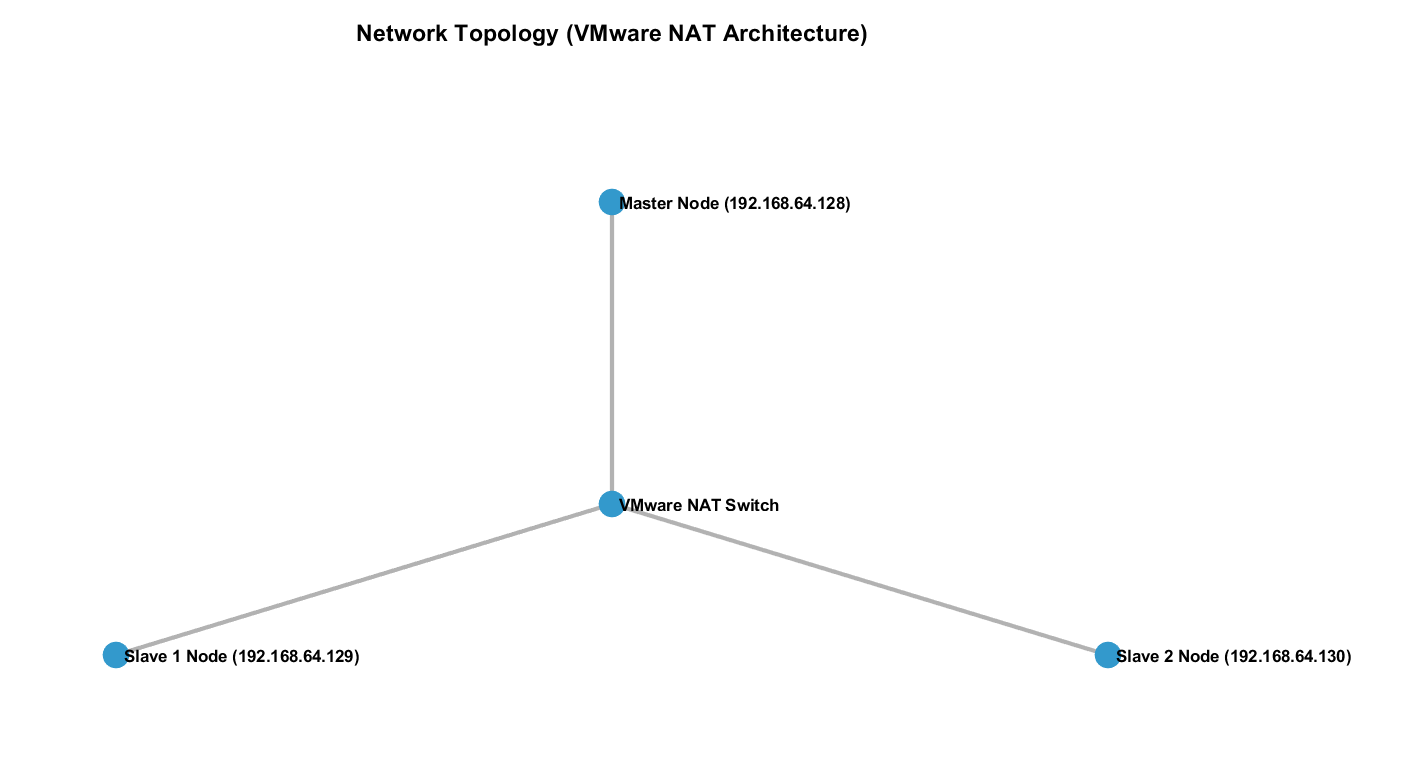
\includegraphics[width=\linewidth,height=.72\textheight,keepaspectratio]{assets/021_p002_01.png}\caption{Diagram or recorded result: Master service and lookup path.}\label{fig:021_p002_010}\end{figure}
\begin{figure}[!htbp]\centering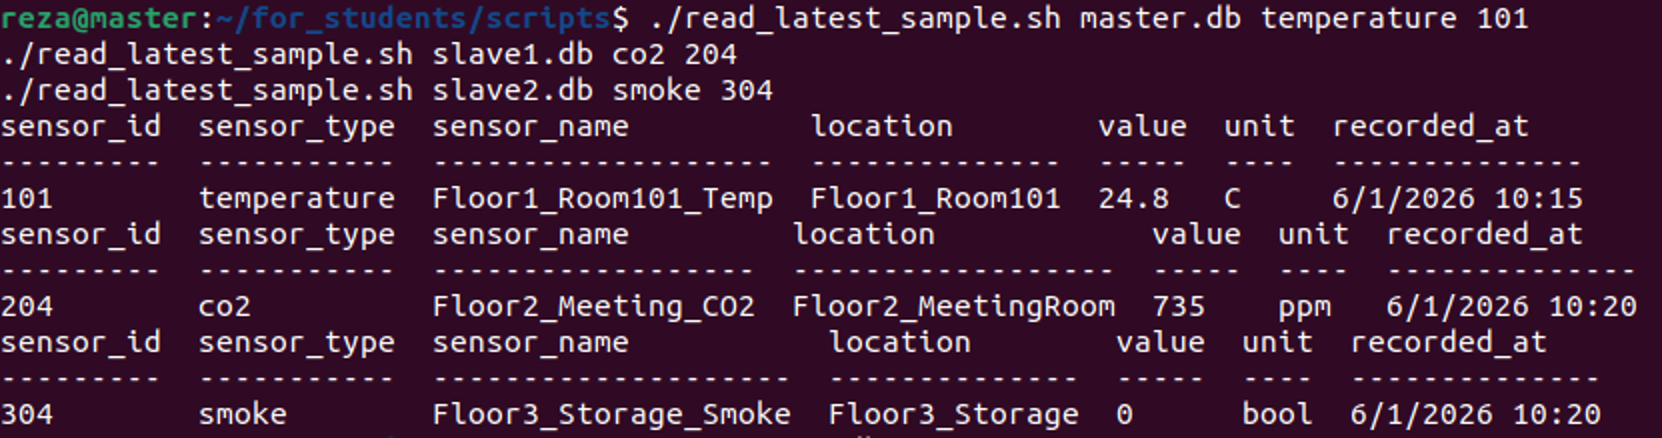
\includegraphics[width=\linewidth,height=.72\textheight,keepaspectratio]{assets/021_p003_01.png}\caption{Diagram or recorded result: Master service and lookup path.}\label{fig:021_p003_010}\end{figure}
\begin{figure}[!htbp]\centering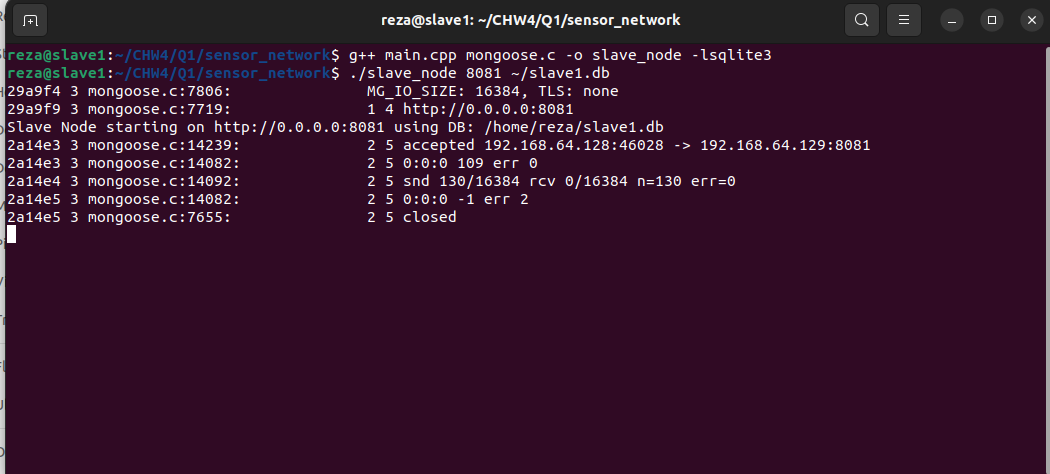
\includegraphics[width=\linewidth,height=.72\textheight,keepaspectratio]{assets/021_p004_01.png}\caption{Diagram or recorded result: Master service and lookup path.}\label{fig:021_p004_010}\end{figure}
\begin{figure}[!htbp]\centering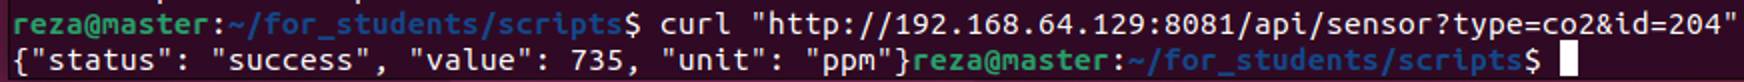
\includegraphics[width=\linewidth,height=.72\textheight,keepaspectratio]{assets/021_p004_02.png}\caption{Diagram or recorded result: Master service and lookup path.}\label{fig:021_p004_020}\end{figure}
\begin{figure}[!htbp]\centering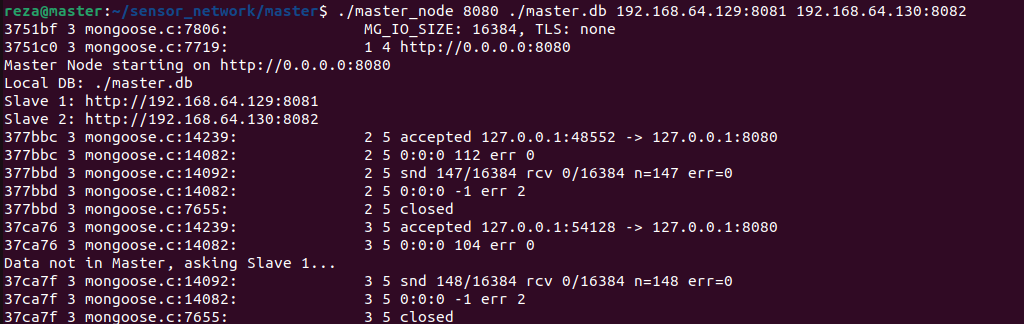
\includegraphics[width=\linewidth,height=.72\textheight,keepaspectratio]{assets/021_p005_01.png}\caption{Diagram or recorded result: Master service and lookup path.}\label{fig:021_p005_010}\end{figure}
\begin{figure}[!htbp]\centering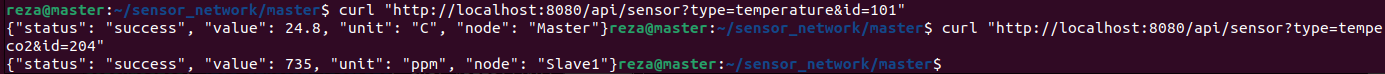
\includegraphics[width=\linewidth,height=.72\textheight,keepaspectratio]{assets/021_p006_01.png}\caption{Diagram or recorded result: Master service and lookup path.}\label{fig:021_p006_010}\end{figure}
\begin{figure}[!htbp]\centering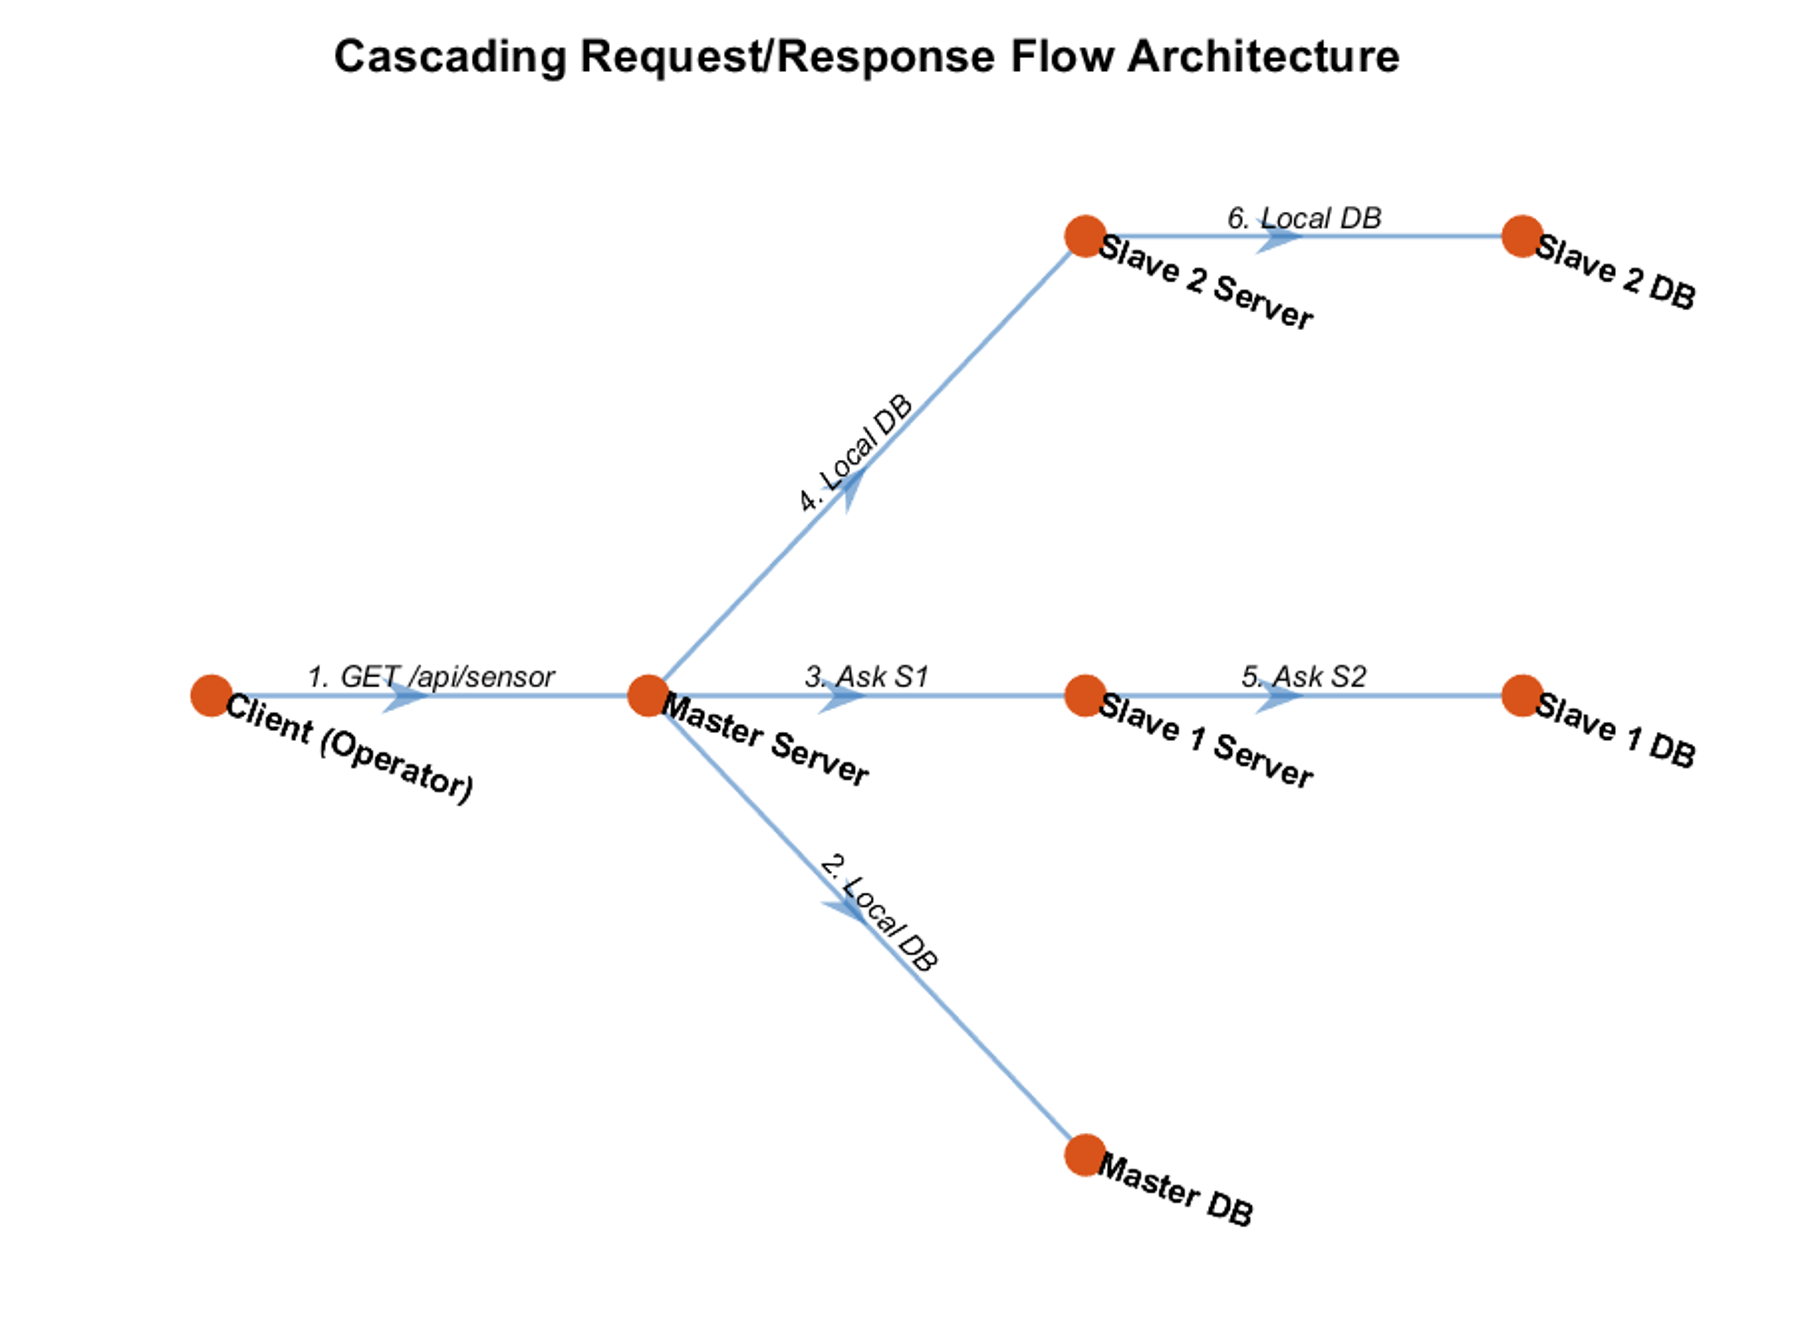
\includegraphics[width=\linewidth,height=.72\textheight,keepaspectratio]{assets/021_p007_01.png}\caption{Diagram or recorded result: Master service and lookup path.}\label{fig:021_p007_010}\end{figure}
\clearpage
\section{Build and test automation}

Separate Makefiles compile master and slave sources and link Mongoose and SQLite. scripts/\allowbreak{}build\_\allowbreak{}and\_\allowbreak{}run.sh clears the previous build, compiles the applications, and displays the master invocation with its arguments. The code directory contains the scripts, Makefiles, and execution instructions for each stage.

\section{Security analysis}

The demonstrated operator/\allowbreak{}master and master/\allowbreak{}slave communication uses plain HTTP. Readings can be observed or modified by an attacker positioned on the network. No application authentication is demonstrated. Although the intended operator path is through the master, exposed slave ports can still accept direct requests unless a firewall prevents them. Further security measures include TLS/\allowbreak{}HTTPS, API-key or bearer-token authentication, firewall rules restricting slave requests to the master, and safe parameterized SQL handling. These remain proposals unless implemented in the source. The report recordedly attributes complete SQL-injection protection to sqlite3\_\allowbreak{}prepare\_\allowbreak{}v2 and sqlite3\_\allowbreak{}bind\_\allowbreak{}text;\allowbreak{} source inspection shows that preparing a concatenated query does not itself provide parameter binding. External values must be bound to placeholders and validated. No single API call justifies a complete-injection-immunity claim.

\section{Two-layer architecture}

Memcached is added to the SQLite-backed nodes. A key identifies a sensor, for example temperature\_\allowbreak{}101. On a request, the service first checks the key. A hit returns the cached value. A miss queries local SQLite or obtains the result from the appropriate downstream node, then stores the successful response with a 60-second TTL before returning it. The main database retains durable readings;\allowbreak{} the cache is temporary and does not replace persistent storage. Expiration can explain a second-round miss if more than 60 seconds pass. Memory pressure and eviction can also remove a key. A current-reading API must consider stale data:\allowbreak{} an insertion or update should invalidate or refresh the matching key, otherwise a reading can remain old until its TTL expires. The experiment report's hit/\allowbreak{}miss path and figures are preserved;\allowbreak{} a fully consistent distributed invalidation policy is not established.

\section{Internal timing and the two-round benchmark}

The application measures response processing using the C+\allowbreak{}+\allowbreak{} chrono facilities. A first-round miss performs database work and possibly an HTTP lookup. A second-round hit obtains the retained result from RAM. The report includes an example described as more than thirteen times faster, and a separate script output with the following observed times. They should be kept as separate observations rather than combined into a single universal speedup.


\begingroup\small\setlength{\tabcolsep}{3pt}\renewcommand{\arraystretch}{1.2}
\begin{longtable}{@{}p{0.2263\linewidth}p{0.2263\linewidth}p{0.2263\linewidth}p{0.2263\linewidth}@{}}
\toprule
\textbf{Read path} & \textbf{First round (ms)} & \textbf{Second round (ms)} & \textbf{Ratio for these observations} \\ \midrule
\endfirsthead
\textbf{Read path} & \textbf{First round (ms)} & \textbf{Second round (ms)} & \textbf{Ratio for these observations} \\ \midrule \endhead
Local reading & 2.4 & 0.08 & 30 \\
Remote example 1 & 21.7 & 0.2 & 108.5 \\
Remote example 2 & 10.2 & 0.2 & 51 \\
\bottomrule\end{longtable}\endgroup

The supplied benchmark is launched from scripts after making benchmark\_\allowbreak{}read.sh executable. It reads the sensors in two rounds and prints the timings. The large ratios show the benefit of serving a retained response in this small experiment. They do not prove that network overhead disappears in general, that every request is a hit, or that the system remains equally fast at scale. Dataset size, cache capacity, workload distribution, expiry, and client concurrency must be reported in a broader evaluation.

\begin{figure}[!htbp]\centering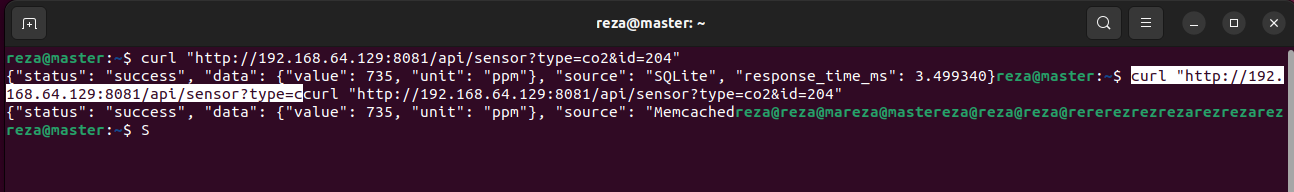
\includegraphics[width=\linewidth,height=.72\textheight,keepaspectratio]{assets/022_p002_01.png}\caption{Diagram or recorded result: Internal timing and the two-round benchmark.}\label{fig:022_p002_010}\end{figure}
\begin{figure}[!htbp]\centering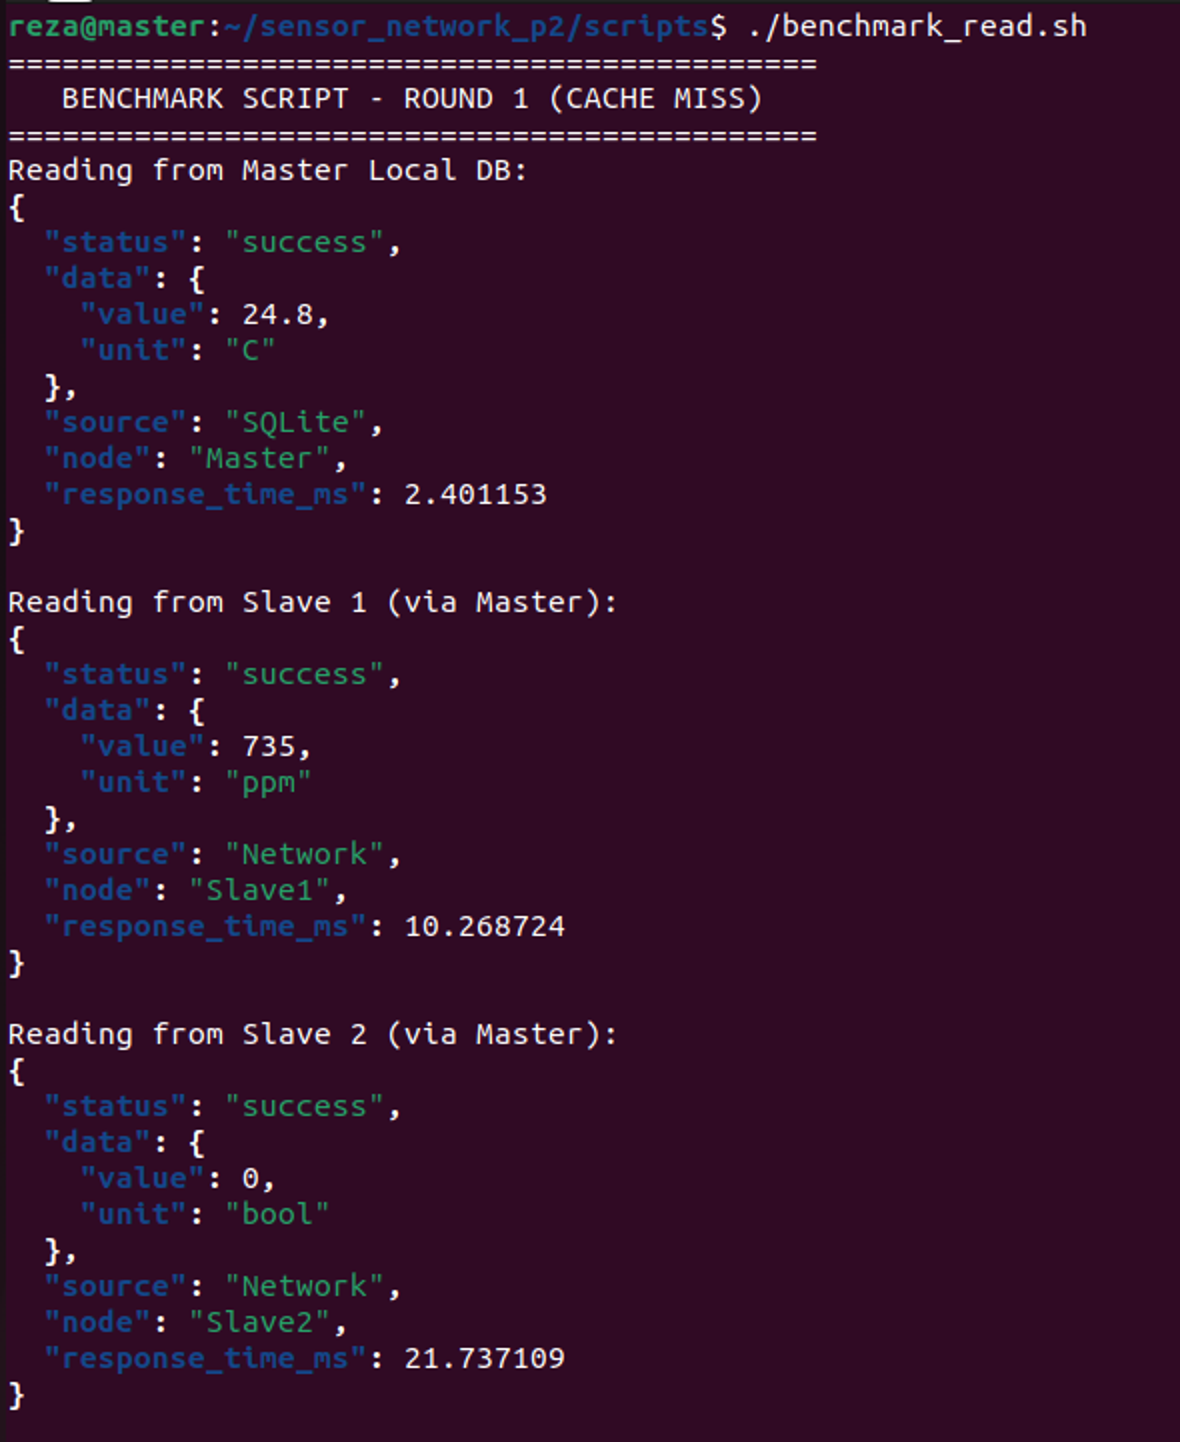
\includegraphics[width=\linewidth,height=.72\textheight,keepaspectratio]{assets/022_p004_01.png}\caption{Diagram or recorded result: Internal timing and the two-round benchmark.}\label{fig:022_p004_010}\end{figure}
\begin{figure}[!htbp]\centering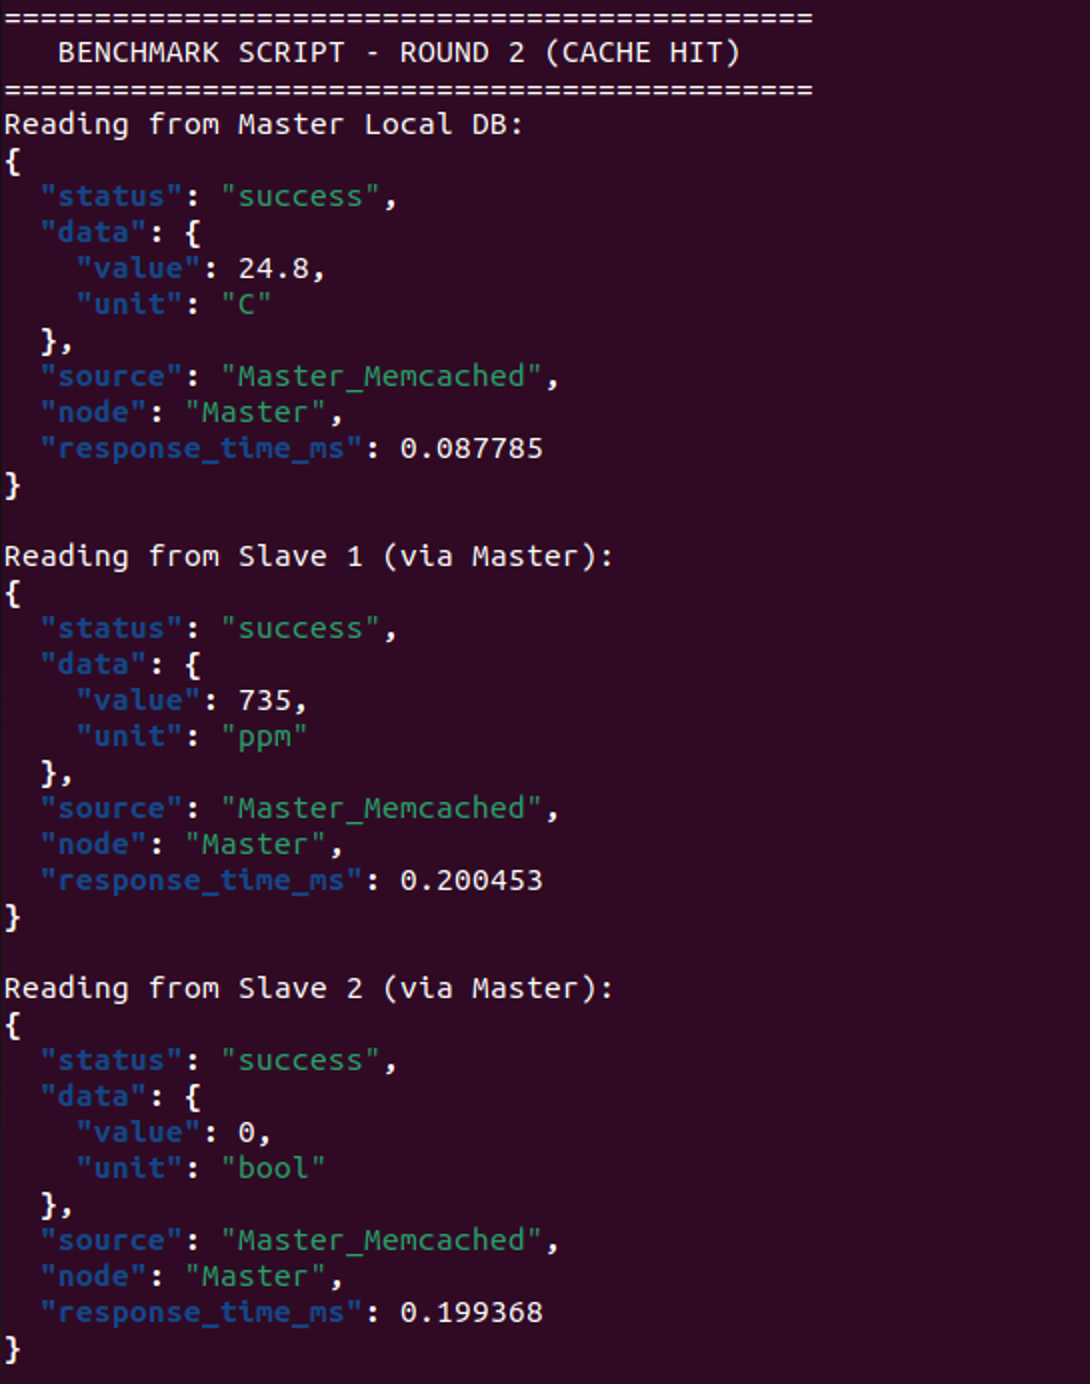
\includegraphics[width=\linewidth,height=.72\textheight,keepaspectratio]{assets/022_p004_02.png}\caption{Diagram or recorded result: Internal timing and the two-round benchmark.}\label{fig:022_p004_020}\end{figure}
\clearpage
\section{Protocol decisions and message path}

The master extends its HTTP service with MQTT publish/\allowbreak{}subscribe request handling. The submission chooses MQTT 3.1.1 for its compact protocol and established support. The recorded argument is that simple sensor lookup does not require version-5 message properties. This is a project choice rather than a claim that version 5 is inappropriate for all embedded systems. QoS 1 is selected as a compromise between delivery acknowledgment and the additional exchange used by QoS 2. It supports at-least-once delivery for the relevant protocol exchange, so duplicate requests and responses should be tolerated. It does not automatically guarantee that an application action is executed once or that a response reaches an unavailable subscriber. The operator communicates through the broker. The master acts as a gateway and performs the cached/\allowbreak{}local/\allowbreak{}remote lookup;\allowbreak{} on a cache miss it can contact the slaves over HTTP.

\begin{figure}[!htbp]\centering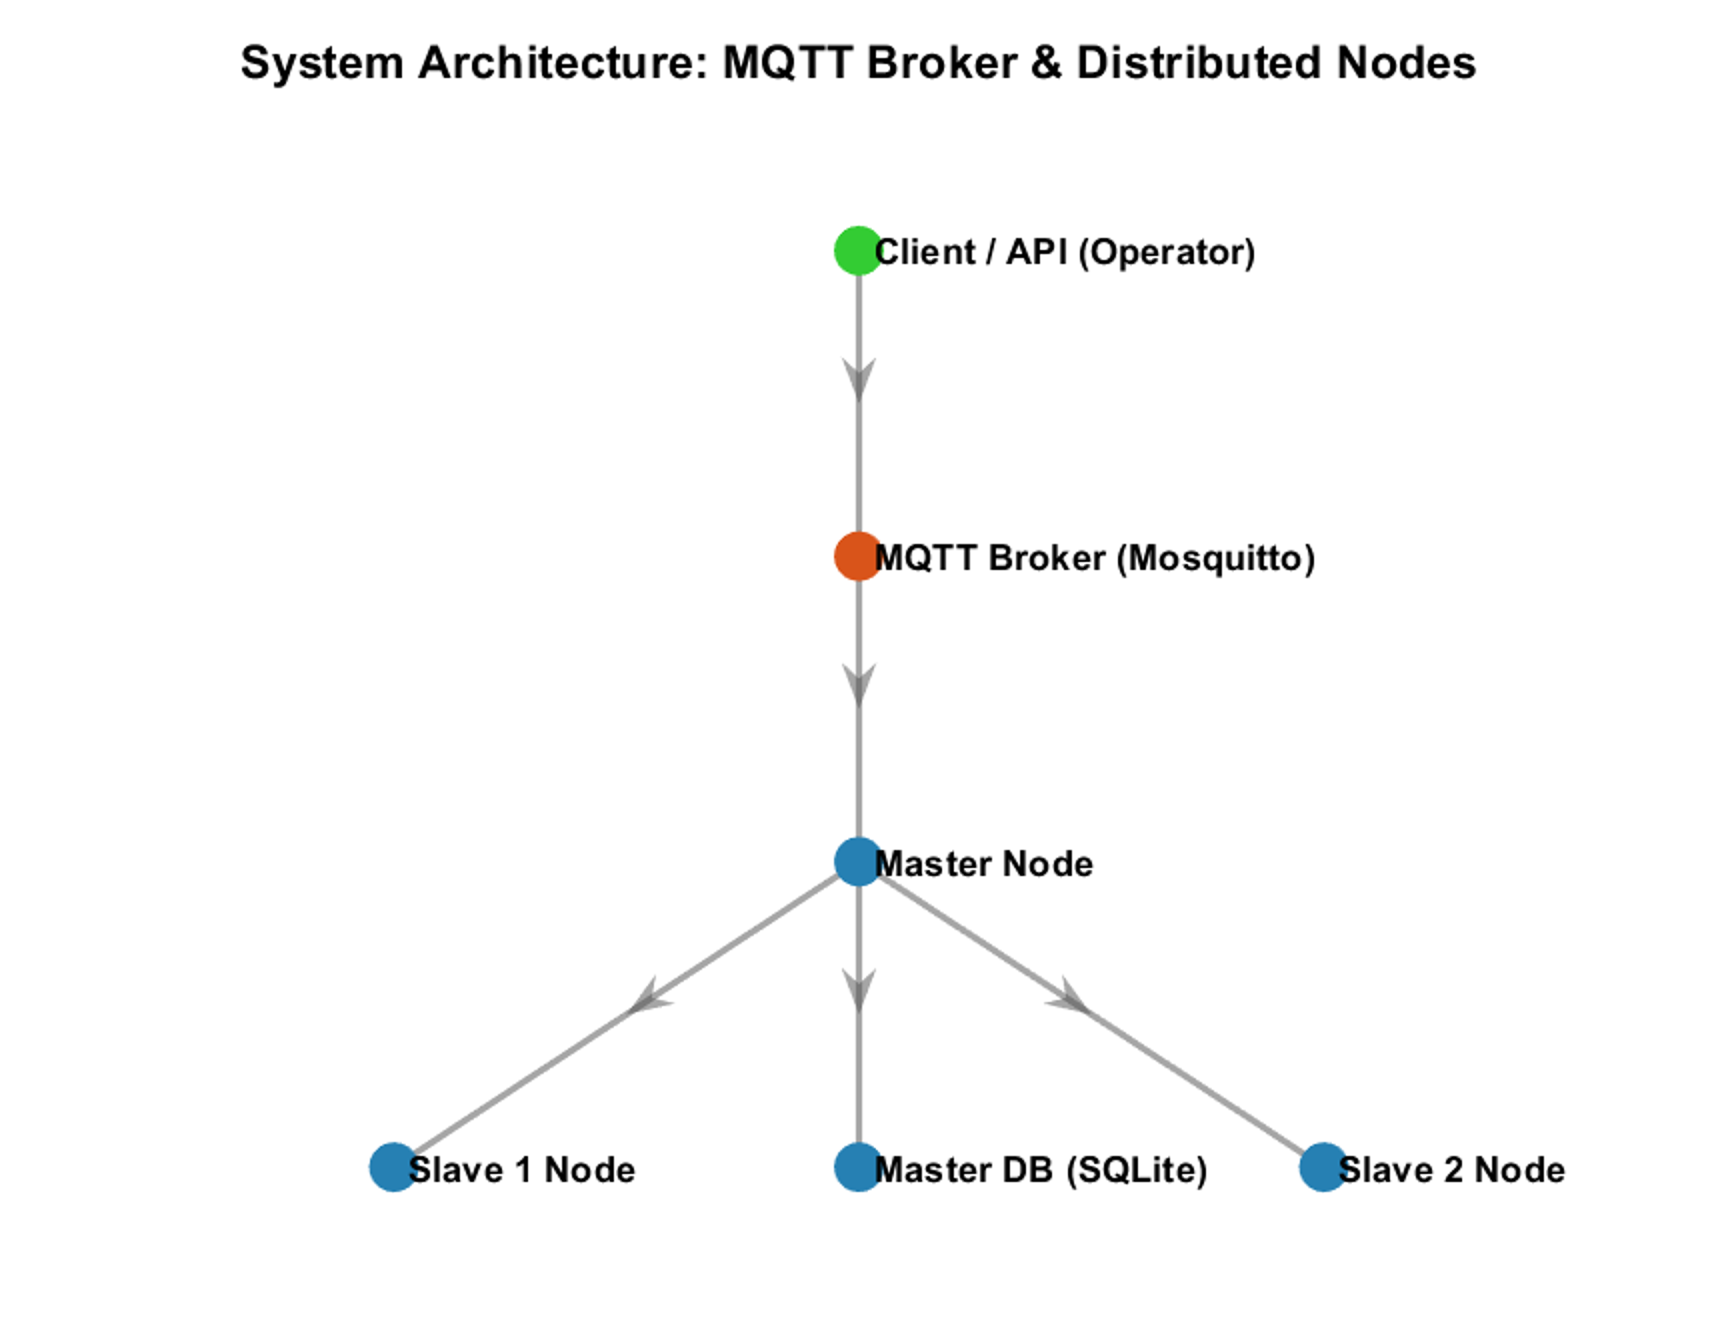
\includegraphics[width=\linewidth,height=.72\textheight,keepaspectratio]{assets/023_p002_01.png}\caption{Diagram or recorded result: Protocol decisions and message path.}\label{fig:023_p002_010}\end{figure}
\begin{figure}[!htbp]\centering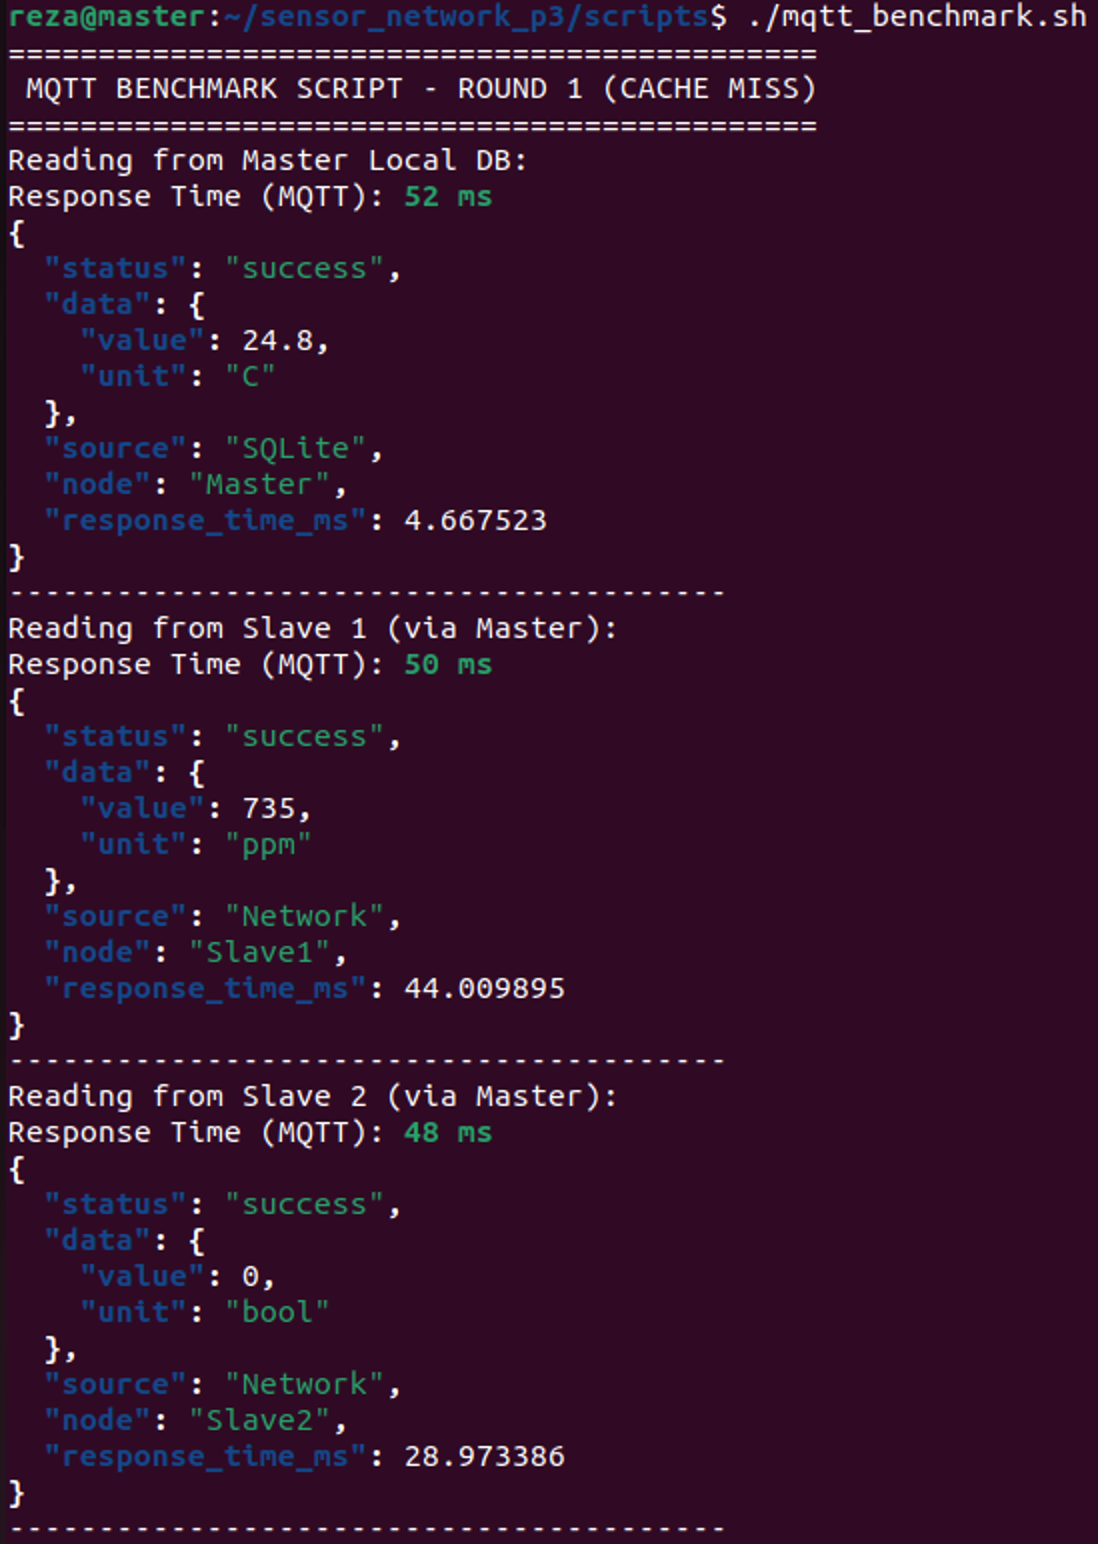
\includegraphics[width=\linewidth,height=.72\textheight,keepaspectratio]{assets/023_p003_01.png}\caption{Diagram or recorded result: Protocol decisions and message path.}\label{fig:023_p003_010}\end{figure}
\begin{figure}[!htbp]\centering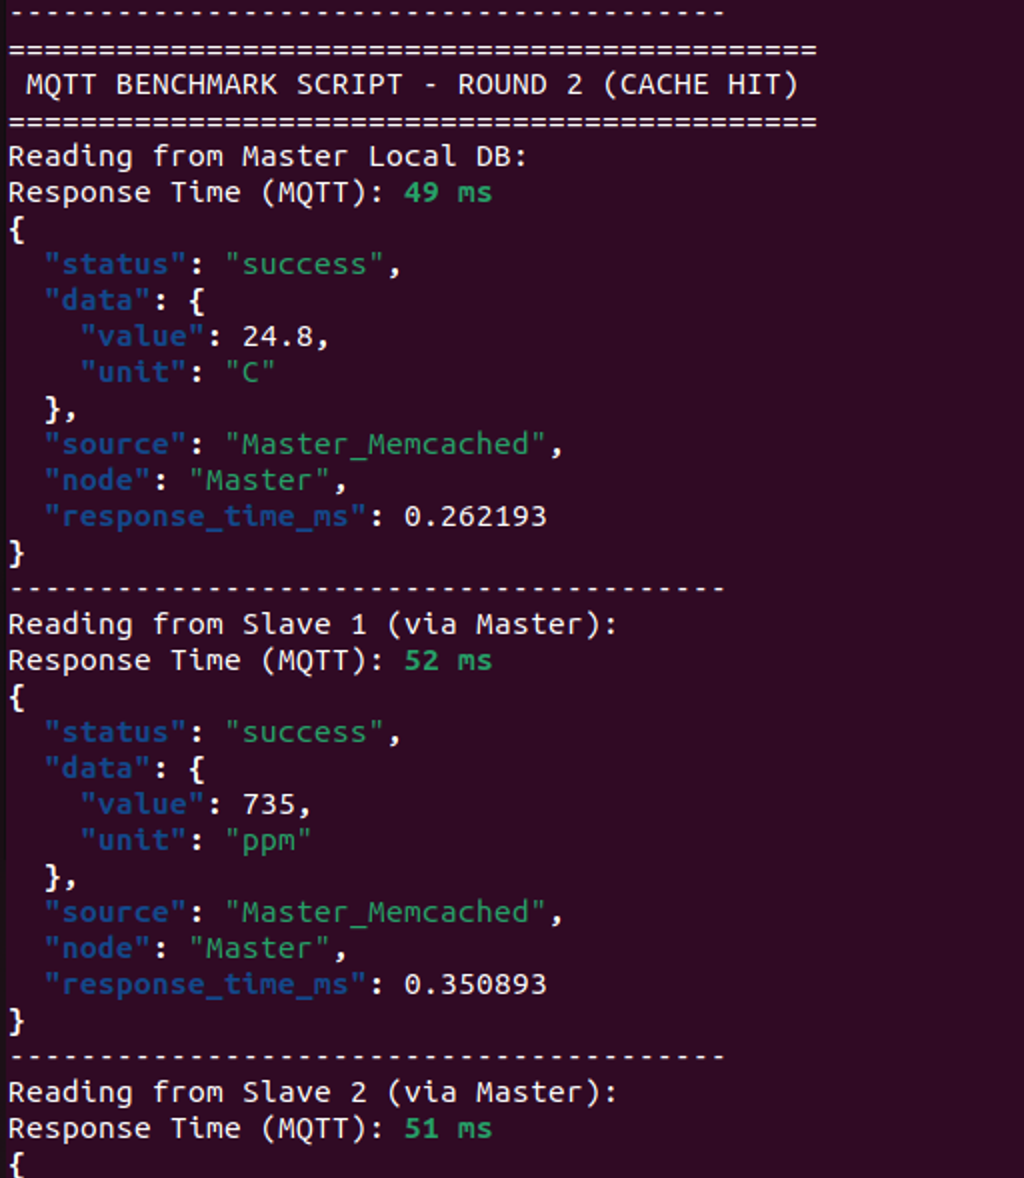
\includegraphics[width=\linewidth,height=.72\textheight,keepaspectratio]{assets/023_p004_01_panel1.png}\caption{Diagram or recorded result: Protocol decisions and message path. Panel 1 of 2.}\label{fig:023_p004_010}\end{figure}

\begin{figure}[!htbp]\centering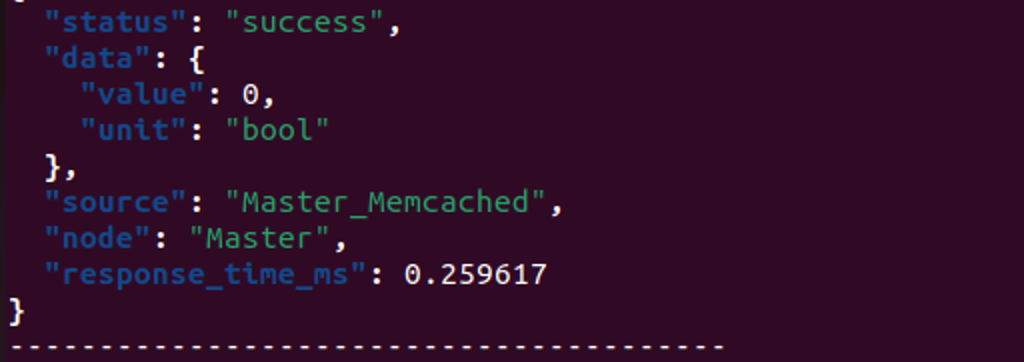
\includegraphics[width=\linewidth,height=.72\textheight,keepaspectratio]{assets/023_p004_01_panel2.png}\caption{Diagram or recorded result: Protocol decisions and message path. Panel 2 of 2.}\label{fig:023_p004_011}\end{figure}
\clearpage
\section{Separating internal service time from total response time}

The output reports two different timings. response\_\allowbreak{}time\_\allowbreak{}ms measures processing within the master, including local SQLite or downstream lookup. First-round examples range from approximately 4.6 to 44 ms;\allowbreak{} second-round cached examples fall to approximately 0.2 ms. The client-observed Response Time includes connection/\allowbreak{}setup, publication, application handling, and response receipt, and remains approximately 48 to 52 ms in both rounds. The cache reduces the internal lookup work, but the reported end-to-end MQTT exchange remains near 50 ms. It is therefore incorrect to apply the internal cache speedup to the complete client path or to infer a bottleneck-free architecture from these few observations. Fixed client overhead, the script's timing method, and broker/\allowbreak{}client scheduling may dominate this workload. The experiment demonstrates protocol integration and different timing boundaries, not a verified large-scale performance result.

\section{Installation and agent configuration}

The master exposes sensor information through snmpd. The recorded installation commands update package metadata and install snmpd, snmp, and jq. A read-only community is configured for local requests. A pass directive binds the illustrative enterprise subtree .1.3.6.1.4.1.55555 to scripts/\allowbreak{}snmp\_\allowbreak{}pass.sh through Bash. The agent is restarted with systemctl after configuration changes. The example subtree is a project-local choice;\allowbreak{} it is not documented as an allocated private enterprise number. SNMPv2c community strings do not provide encrypted, cryptographically authenticated monitoring. Restrict access appropriately in a reproduction and consider SNMPv3 for a deployment requiring those properties.

\section{OID structure}

Each demonstrated sensor has entries for name, type/\allowbreak{}description, and latest value. The master temperature sensor 101 uses suffixes .1.1, .1.2, and .1.3 under the chosen root. Slave-1 CO2 sensor 204 uses .2.1 through .2.3. Slave-2 smoke sensor 304 uses .3.1 through .3.3. This organization is retained from the experiment report and configuration.

\begin{figure}[!htbp]\centering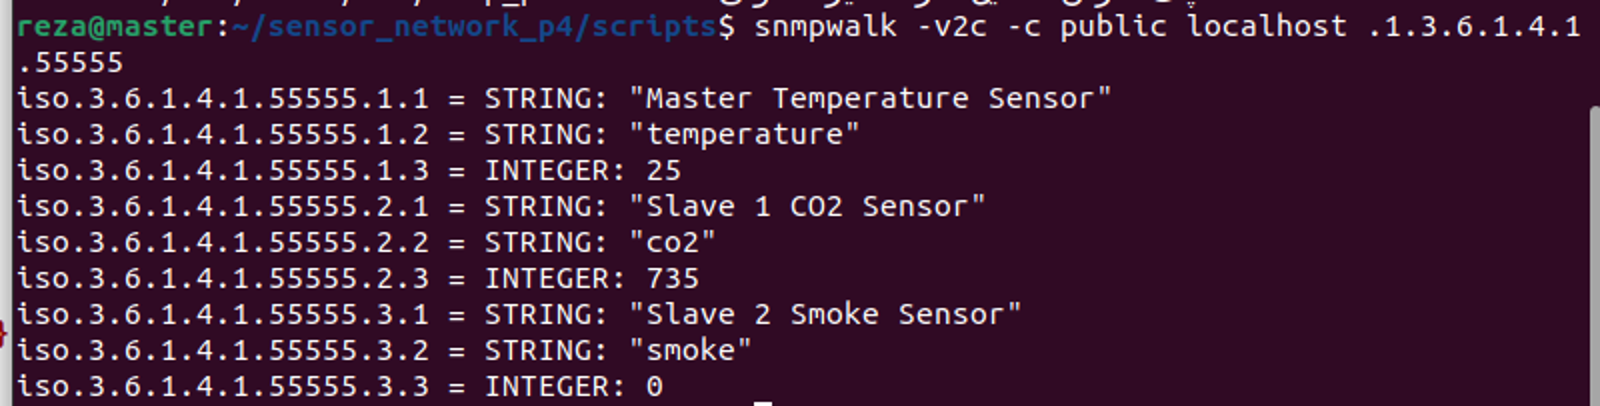
\includegraphics[width=\linewidth,height=.72\textheight,keepaspectratio]{assets/024_p002_01.png}\caption{Diagram or recorded result: OID structure.}\label{fig:024_p002_010}\end{figure}
\clearpage
\section{Request-to-response flow}

The operator walks the subtree with snmpwalk using version 2c. snmpd invokes the pass script with the requested OID. The script sends an HTTP request with curl to the master API on its configured port, rather than directly reading an unrelated database. The master then retrieves the reading through the existing cache/\allowbreak{}local/\allowbreak{}remote path. The script prints the result in the format expected by the SNMP adapter and snmpd returns it to the client. The all-sensor test is run by making read\_\allowbreak{}snmp.sh executable and launching it from scripts. This architecture reuses the HTTP lookup contract, but its performance and availability also depend on that service;\allowbreak{} the existence of an SNMP adapter does not eliminate the master as a central dependency.

\section{Route and query contract}

The Mongoose service provides /\allowbreak{}api/\allowbreak{}sensor/\allowbreak{}logs. It accepts sensor\_\allowbreak{}name, sensor\_\allowbreak{}id, and date in YYYY-MM-DD format. A request first reaches the master, which searches its local database. If no matching history is present, it forwards the request to slave services and returns their structured result. Local and remote database rows are not fabricated from fixed examples. The report illustrates selecting time(recorded\_\allowbreak{}at) and value from sensor\_\allowbreak{}readings for a specified calendar date. A complete implementation also identifies the requested sensor and uses parameter binding for caller-supplied inputs. Date format, missing parameters, empty histories, invalid identifiers, and network failures need distinguishable behavior.

\begin{figure}[!htbp]\centering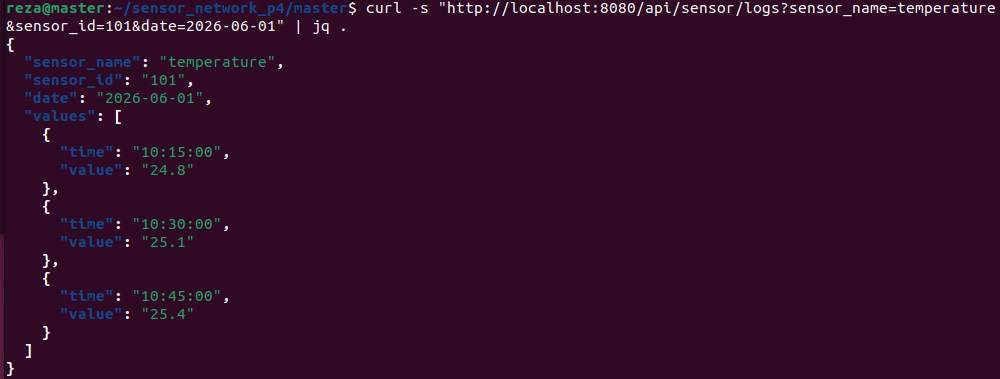
\includegraphics[width=\linewidth,height=.72\textheight,keepaspectratio]{assets/025_p002_01.png}\caption{Diagram or recorded result: Route and query contract.}\label{fig:025_p002_010}\end{figure}
\begin{figure}[!htbp]\centering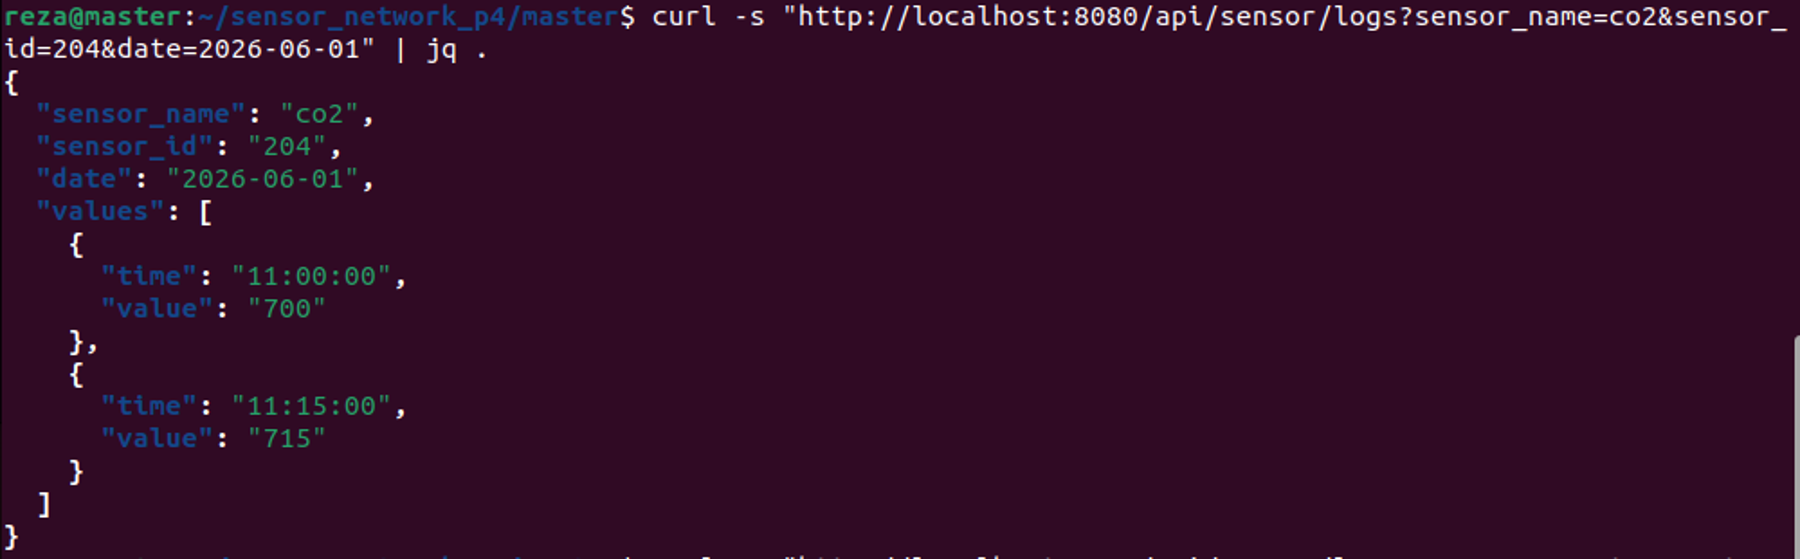
\includegraphics[width=\linewidth,height=.72\textheight,keepaspectratio]{assets/025_p003_01.png}\caption{Diagram or recorded result: Route and query contract.}\label{fig:025_p003_010}\end{figure}
\begin{figure}[!htbp]\centering
\includegraphics[width=\linewidth,height=.72\textheight,keepaspectratio]{assets/025_p003_02.png}\caption{Diagram or recorded result: Route and query contract.}\label{fig:025_p003_020}\end{figure}
\clearpage
\section{Submitted tests}

The first test requests the master's temperature-sensor history on 2026-06-01. The second requests CO2 history located on slave 1 through the master. The third requests an absent date, 2020-01-01, and receives a defined no-data response. These cases demonstrate local lookup, remote lookup, and an empty-result path;\allowbreak{} they do not establish exhaustive validation or all network-error behavior. Returned JSON identifies the sensor/\allowbreak{}date and contains an array of time/\allowbreak{}value entries. Timezone and ordering should be explicit in a production contract, because interpreting a calendar day through SQLite date functions can differ from an operator's intended local day.

\section{Background service and monitoring loop}

The alert process runs independently under systemd. Every five seconds it retrieves the newest available record for each sensor and compares its time/\allowbreak{}value with the configured rules. SQLite is configured in WAL mode to improve overlap between reading and writing. WAL reduces some contention but does not guarantee an absence of locks, unlimited concurrent writers, or immunity to busy errors. Before inserting an alert, the program checks for a matching outstanding event with status NEW. If one exists, it avoids inserting the same active condition again. This bounds repeated alerts while preserving a persistent record that requires acknowledgment. A complete lifecycle would define transitions such as acknowledgment and resolution;\allowbreak{} they are not inferred from the duplicate-suppression mechanism alone.

\section{Trigger rules}

\begingroup\small\setlength{\tabcolsep}{3pt}\renewcommand{\arraystretch}{1.2}
\begin{longtable}{@{}p{0.4775\linewidth}p{0.4775\linewidth}@{}}
\toprule
\textbf{Alert type} & \textbf{Recorded rule} \\ \midrule
\endfirsthead
\textbf{Alert type} & \textbf{Recorded rule} \\ \midrule \endhead
TIMEOUT\_\allowbreak{}NO\_\allowbreak{}DATA & Latest known reading is older than 300 seconds \\
INVALID\_\allowbreak{}DATA & Reading below -50 or above 1000 \\
HIGH\_\allowbreak{}TEMPERATURE & Temperature above 40 C \\
HUMIDITY\_\allowbreak{}OUT\_\allowbreak{}OF\_\allowbreak{}BOUNDS & Humidity below 20 percent or above 80 percent \\
\bottomrule\end{longtable}\endgroup

These thresholds document the submitted configuration, not universal limits for every sensor. In particular, units and admissible ranges must be associated with sensor type. A query based only on existing readings cannot detect an expected sensor that has never produced a row;\allowbreak{} detecting that case requires joining the sensor registry to its readings.

\begin{figure}[!htbp]\centering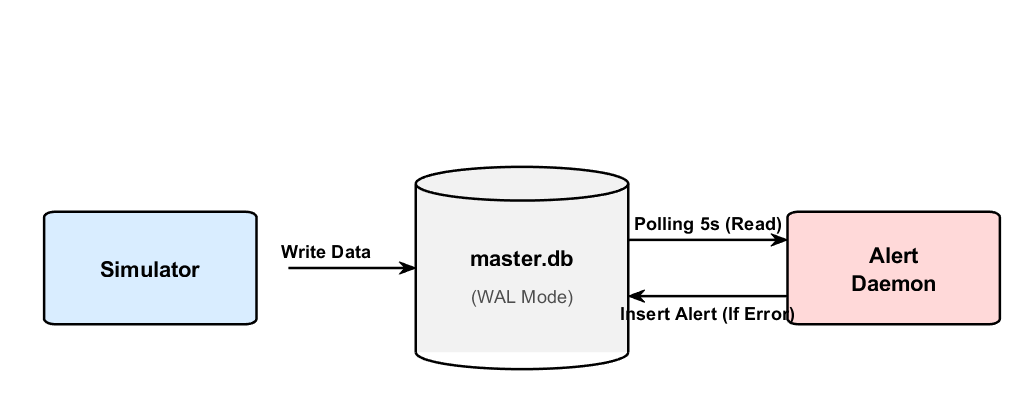
\includegraphics[width=\linewidth,height=.72\textheight,keepaspectratio]{assets/026_p001_01.png}\caption{Alert-service architecture: Trigger rules.}\label{fig:026_p001_010}\end{figure}
\begin{figure}[!htbp]\centering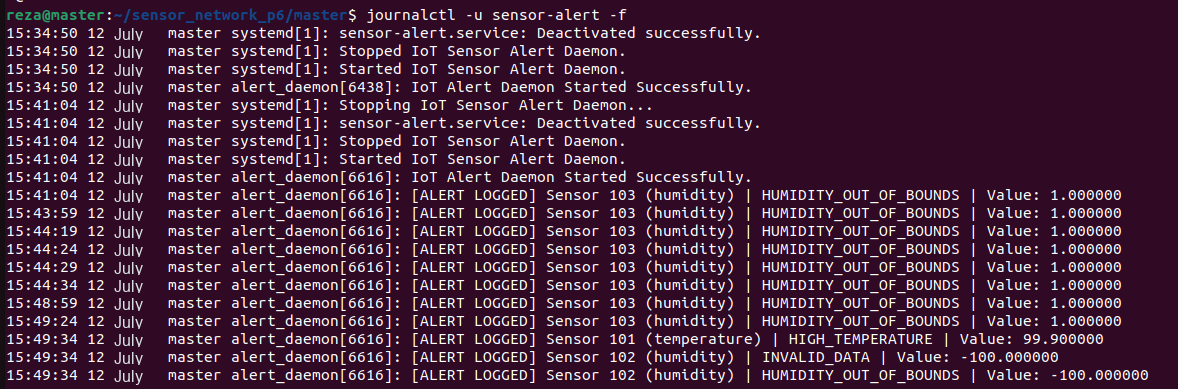
\includegraphics[width=\linewidth,height=.72\textheight,keepaspectratio]{assets/026_p002_01.png}\caption{Diagram or recorded result: Trigger rules.}\label{fig:026_p002_010}\end{figure}
\begin{figure}[!htbp]\centering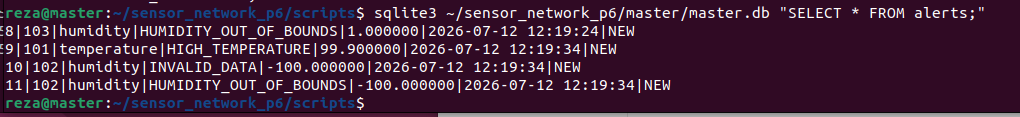
\includegraphics[width=\linewidth,height=.72\textheight,keepaspectratio]{assets/026_p003_01.png}\caption{Diagram or recorded result: Trigger rules.}\label{fig:026_p003_010}\end{figure}
\begin{figure}[!htbp]\centering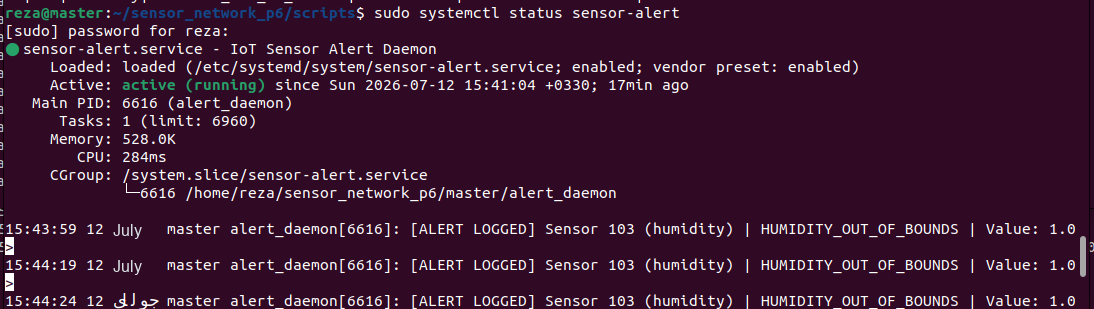
\includegraphics[width=\linewidth,height=.72\textheight,keepaspectratio]{assets/026_p004_01.png}\caption{Implementation and output: Trigger rules.}\label{fig:026_p004_010}\end{figure}
\clearpage
\section{Persistent alert schema}

The alerts table has an increasing integer primary key id;\allowbreak{} sensor\_\allowbreak{}id;\allowbreak{} sensor\_\allowbreak{}name;\allowbreak{} alert\_\allowbreak{}type;\allowbreak{} sensor\_\allowbreak{}value;\allowbreak{} a created\_\allowbreak{}at timestamp;\allowbreak{} and status, initially NEW. It records the value observed when the rule is triggered and gives an operator a durable list to inspect.

\section{Delivery and scope}

The source is implemented in C+\allowbreak{}+\allowbreak{}. The submission includes a combined master build script, a service-installation/\allowbreak{}start script, and a database initializer that creates the alert table and enables WAL. The daemon monitors the configured local master database. The evidence does not demonstrate automatic monitoring of every slave database, every expected sensor, or complete node-failure coverage. The English report distinguishes this implemented scope from the broader monitoring objective instead of claiming a distributed alert capability that has not been established.

\end{document}